\chapter{背景}\label{chapter_background}

本节将介绍本文的测试对象:安卓服务以及安卓广播接收器。
\section{安卓服务}

在安卓系统中,每个安卓应用都对应着一个主线程,这个主线程将负责处理界面计算和渲染、负责处理用户的交互以及负责响应生命周期事件等。这些任务对主线程产生了快速响应的要求,否则会导致用户体验质量的下降。换言之,在主线程中只能进行不耗时(几毫秒级别)的计算和操作,而任何耗时较长的计算和操作都必须在主线程之外的单独的后台线程之上来完成。这样可以使得用户在积极的与应用交互时,应用在后台可以积极的响应和运行。

然而,后台任务不可避免地将会使用安卓设备的资源:例如内存资源和电池电量等。如果后台任务操作不当(如占用大量内存导致系统卡顿,长期进行密集计算导致电池电量下降变快),也可能会导致用户体验下降;同时如果安卓服务的开发人员在开发时引入了\textbf{程序缺陷},使得服务在运行时产生了\textbf{内存泄漏},将会使得前面的现象变得更加严重。因此随着安卓系统的更新,其对服务组件也进行了更多的限制,以尽可能保证用户体验。

\begin{itemize}
	\item \textbf{安卓6.0(API 级别 23) } 引入了\textbf{低电量模式以及应用待机模式}。低电量模式会在屏幕关闭且设备处于静止状态时,对运行中应用的行为进行限制,以减少电量消耗,例如:限制网络访问,限制同步等。即当开启低电量模式时,服务的行为会受到一定程度的限制。
	\item \textbf{安卓7.0(API 级别 24)} 此版本限制了隐式广播的注册,并将上个版本中推出的低耗电模式推广成为一个随时进行的系统耗电优化:即当屏幕一段时间处于未唤醒状态且未接入电源,低耗电模式就会启动,而无需手动开启。即只要设备处于闲置状态时,服务的行为随时都会受到限制。
	\item \textbf{安卓8.0(API 级别 26)} 对后台服务的行为进行了更严格的限制,其中影响较大的一条规则是:\textbf{禁止处于后台的应用启动新的服务},取而代之的是需要显式经过用户许可,启动前台服务。这些限制对跨应用测试的研究带来了不便(跨应用测试一般由测试人员编写的测试驱动应用去启动其他(后台)应用的组件)。
	\textbf{安卓9.0(API 级别 28)} 引入了应用待机存储分区。系统将会根据应用的使用模式,来动态分配给应用使用资源的优先级。
\end{itemize}

本节接下来将会详细介绍服务的启动方式,生命周期,注册方式,以及内存泄漏的成因。

\subsection{服务的启动方式}
安卓应用中的服务可以通过两种方式启动\cite{service}:

\textbf{start 方式 } 其他组件构造特定的\textbf{Intent}对象,通过调用\textbf{startService() API}来启动目标服务。

\textbf{bind 方式 } 通过调用\textbf{bindService() API}将目标服务与特定组件绑定。被绑定的服务提供接口供其他组件与之交互。
一个服务可以同时通过以上两种方式启动。

\subsection{服务的生命周期}
服务的生命周期根据启动方式不同分为两种\cite{service}:

\textbf{start 方式 } 通过\textbf{startService() API}启动的服务将会一直运行,直到调用\textbf{stopSelf()}方法将自己停止运行。其他组件也可以通过调用\textbf{stopService() API}将服务停止运行。

停止运行的服务将会被\textbf{GC(Garbage Collector)}回收。

\textbf{bind 方式 } 通过\textbf{bindService() API}启动的服务将通过\textbf{IBinder}接口与其他组件进行交互,直到其他组件调用\textbf{unbindService() API}解除绑定。

一个服务可以同时绑定到多个组件之上,直到所有组件都解除了绑定时,该服务才会被\textbf{GC}回收。

每个安卓应用都关联一个\textbf{ActivityThread}实例,负责调度和执行该应用的各种组件。\textbf{ActivityThread}有一个\textbf{ArrayMap}类型的成员变量\textbf{mServices},其中保存了所有没有被销毁的服务的引用。一旦某个服务的实例被销毁,其引用将会从\textbf{mServices}中删除。

\subsection{服务的注册方式}
\begin{listing}[htbp]
	\centering
	\caption{服务的注册方式}
	\begin{minted}[encoding=utf8,
	frame=single,
	framesep = 1em,
	numbers=left, 
	breaklines=true, 
	tabsize=4,
	xleftmargin=2em,xrightmargin=2em,
	fontsize=\footnotesize]{xml}
<manifest
	xmlns:android="http://schemas.android.com/apk/res/android"
	xmlns:dist="http://schemas.android.com/apk/distribution"
	package="com.example.myapplication">
	<dist:module dist:instant="true" />
	<application ...>
		...
		<service android:name=".Service1"
			android:enabled="true"
			android:exported="true">
		</service>
		<service
			android:name = ".Service2"
			android:enabled = "true"
			android:exported = "false">
			<intent-filter>
				<category android:name = "cat1"/>
				<action android:name = "act2"/>
			</intent-filter>
		</service>
		<service android:name = ".Service3"
			android:enabled = "true"
			android:permission = "Permission1">
			<intent-filter>
				<action android:name = "act3"/>
				<category android:name = "cat2"/>
				<data android:scheme = "Scheme1"/>
				<data android:scheme = "Scheme2"/>
			</intent-filter>
		</service>
	</application>
</manifest>
	\end{minted}
	\label{declaration:service}
\end{listing}
通常,每个服务都要在\textbf{AndroidManifest.xml}中注册一个\textbf{<service>}标签(参考Listing.\textcolor{red}{\ref{declaration:service}}中的样例)。同时服务可以通过设置"\textbf{android:exported}"属性来指定该服务是否将被导出。当设置\textbf{android:exported = "true"}时,该服务可以被其他应用使用,反之不可。
%可以凑更多字数
\subsection{服务的内存泄漏}\label{service_leak}
通常,一个服务的实例不再被使用时应该被\textbf{GC(Garbage Collector)}回收,并释放资源。然而在某些情况下,一个被销毁的服务可能会意外的被引用,从而使得\textbf{GC}无法将其回收并释放资源,这样就造成了服务的内存泄漏。
\begin{listing}[htbp]
	\centering
	\caption{服务的内存泄漏}
	\begin{minted}[encoding=utf8,
	frame=single,
	framesep = 1em,
	numbers=left, 
	breaklines=true, 
	tabsize=4,
	showtabs = false,
	xleftmargin=2em,xrightmargin=2em,
	fontsize=\footnotesize]{java}
public class LeakedService extends Service{
	private static final String TAG = "LeakedService";
	// Method will be called when an instance is creating.
	public void onCreate(){
		...
		new Timer().scheduleAtFixedRate(new TimerTask(){
			public void run(){
				Log.d(TAG, LeakedService.this.getPackageName() + ".LeakedService is running!");
			}
		},1000L,3000L);
	}
	// Method will be called when an instance is destroying.
	public void onDestroy(){
		...
	}
}
	\end{minted}
	\label{leaked example:service}
\end{listing}

例如在游戏\emph{com.siendas.games2048}中,就出现了原理如图(见\textbf{Listing.\textcolor{red}{\ref{leaked example:service}}})的内存泄漏。具体导致内存泄露的原理为:在\textbf{LeakedService}的实例被构造的时候,将会调用他的\textbf{onCreate()}方法,在该方法中延迟\textbf{1000ms}启动了一个\textbf{匿名}计时器,该计时器将以\textbf{3000ms}的周期打印调试信息,可以看到在\textbf{TimerTask}类中持有了\textbf{LeakedService}的引用,而在该服务被销毁时,其\textbf{onDestroy()}方法中并没有对该匿名计时器进行销毁。因此在该服务被销毁后,将会一直存在一个匿名计时器持有该服务的引用,导致\textbf{GC}无法将其回收,从而导致了内存泄漏。

\section{安卓广播接收器}

安卓系统中,可以在安卓应用之间、以及安卓应用与安卓系统之间实现通讯,这种通讯的手段被称为广播\cite{androidbroadcastsguide},广播的设计采用了发布-订阅的设计模式。特定的广播将会在特定的事件发生时发送,例如:安卓系统将在各种系统事件(插拔耳机,插拔电源等)发生时发送系统广播;再如:一个安卓应用可以发送自定义的广播来同志其他的安卓应用,将一些消息传递给后者。

在使用广播时,应用需要注册接收特定的广播(称之为\textbf{订阅订阅})。在相应的广播发出,将由安卓系统负责将广播发送给订阅此种广播的应用。因此在安卓应用的角度,只需要订阅所需要的广播类型,以及关注在接收到广播时需要做出的响应动作即可,具有这种功能的组件被称为\textbf{广播接收器}。
	
一般而言,在跨应用通信时,广播是被广泛使用的一种方便的手段。但是在使用广播时需要格外小心,如果应用滥用广播,可能会导致系统运行变迟钝。更严重的,如果开发人员在编写广播接收器的时候引入\textbf{程序缺陷},将会导致更严重的问题(如应用崩溃等)。

本节接下来将会介绍广播接收器的启动方式,生命周期,注册方式,以及内存泄漏的成因。

\subsection{广播接收器的启动方式}
安卓应用中的广播接收器亦有两种方式启动\cite{broadcast}:

\textbf{清单声明的接收器 }\label{declaration:receiver in manifest} 通过在\textbf{AndroidManifest.xml}中添加\textbf{<receiver>}标签注册广播接收器,通过\textbf{<intent-filter>}标签指定接收器所订阅的广播操作。系统软件包管理器会在应用安装时注册接收器。然后,该接收器会成为应用的一个独立入口点,这意味着如果应用当前尚未运行,系统可以启动应用并发送广播。系统会创建新的\textbf{BroadcastReceiver}组件对象来处理它接收到的每个广播。次对象仅在调用\textbf{onReceive(Context, Intent)}期间有效。一旦从此方法返回代码,系统便会认为该组件不再活跃。

\textbf{上下文注册的接收器 }\label{declaration:receiver in context} 通过在代码中构造出\textbf{BroadReceiver}实例,以及\textbf{IntentFilter}实例来指定订阅的广播内容,调用\textbf{registerReceiver(BroadcastReceiver, IntentFilter) API}来注册接收器。只要上下文有效,通过改种方式注册的广播接收器就会接收广播。如果要停止接收广播,需要调用\textbf{unregisterReceiver(BroadcastReceiver) API}来注销广播接收器

\subsection{广播接收器的生命周期}

广播接收器的生命周期根据启动方式不同亦分为两种\cite{broadcast}:

\textbf{清单声明的接收器 } 静态注册的接收器生命周期不限于\textbf{Activity}甚至整个应用。即使应用并不在运行,接收器也可以接收到订阅的广播。将会在\textbf{onReceive()}方法结束后被销毁。


\textbf{上下文注册的接收器 } 上下文注册的接收器,其生命周期仅限于注册的上下文,例如在\textbf{Activity}上下文注册的接收器,在整个\textbf{Activity}存活期间可以持续接收广播;在应用上下文中注册的接收器,则会在整个应用运行期间都可以接收广播。需要注意的是:这种方式启动的接收器必须手动进行销毁,即调用\textbf{unregisterReceiver() API},否则在上下文失效时,系统会抛出异常(并不会导致应用崩溃),同时接收器会引发泄露(见图.\textcolor{red}{\ref{fig:broadcast_leak}})。

\begin{figure}[htbp]
	\centering
	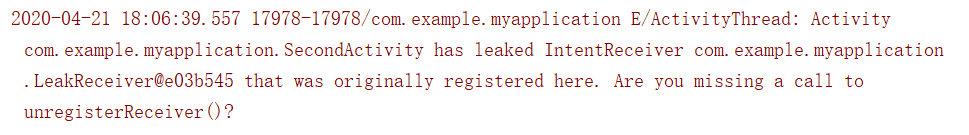
\includegraphics[width=0.9\textwidth]{broadcast_leak.png} % requires the graphicx package
	\caption{没有回收接收器将会导致异常以及泄露}
	\label{fig:broadcast_leak}
\end{figure}

\subsection{广播接收器的注册方式}
\begin{listing}[htbp]
	\centering
	\caption{广播接收器的注册方式}
	\begin{minted}[encoding=utf8,
	frame=single,
	framesep = 1em,
	numbers=left, 
	breaklines=true, 
	tabsize=4,
	showtabs = false,
	xleftmargin=2em,xrightmargin=2em,
	fontsize=\footnotesize]{XML}
<manifest 
	xmlns:android="http://schemas.android.com/apk/res/android"
	xmlns:dist="http://schemas.android.com/apk/distribution"
	package="com.example.myapplication">
	<dist:module dist:instant="true" />
	<application ...>
		...
		<receiver
			android:name = ".Receiver1">
			<intent-filter>
				<action android:name = "act1" />
			</intent-filter>
		</receiver>
		<receiver
			android:name = ".Receiver2"
			android:exported = "false"
			android:enabled = "true">
			<intent-filter>
				<category android:name = "cat1" />
				<action android:name = "act2" />
			</intent-filter>
		</receiver>
	</application>
</manifest>
	\end{minted}
	\label{declaration:receiver}
\end{listing}

一般而言,清单声明的广播接收器(见\ref{declaration:receiver in manifest})需要在\textbf{AndroidManifest.xml}文件中添加\textbf{<receiver>}标签(参考\textbf{Listing.\textcolor{red}{\ref{declaration:receiver}}}),在\textbf{<intent-filter>}子标签中可以指定订阅的广播内容等,也可以通过设置\textbf{"android:exported"}属性来指定该广播是否将被导出。而上下文注册的广播接收器(见\ref{declaration:receiver in context})则不需要进行前文的操作。
\subsection{广播接收器的内存泄漏}
广播接收器的内存泄漏原理类似与服务内存泄漏\ref{service_leak}。但是由广播接收器引起的内存泄漏往往比服务更为严重,因为广播接收器被系统认为只进行不耗时的操作(如果超过10s未从\textbf{onReceive()}方法中返回,将抛出\textbf{ANR Exception}),因此通常广播接收器在接到广播后,很有可能会启动其他的\textbf{Service}进行后续的耗时操作,进而可能会导致一连串的内存泄漏。

例如图中(见\textbf{Listing.\textcolor{red}{\ref{leaked example:receiver}}})所示的广播接收器,不仅本身会导致内存泄漏,而且还会启动一个会导致内存泄漏的服务(见\textbf{Listing.\textcolor{red}{\ref{leaked example:service}}}),因此后果将会更加严重。
\begin{listing}[htbp]
	\centering
	\caption{广播接收器的内存泄漏}
	\begin{minted}[encoding=utf8,
	frame=single,
	framesep = 1em,
	numbers=left, 
	breaklines=true, 
	tabsize=4,
	showtabs = false,
	xleftmargin=2em,xrightmargin=2em,
	fontsize=\footnotesize]{java}
public class LeakReceiver extends BroadcastReceiver {
	private final String TAG = "LeakReceiver";
	private final int ID = new Random().nextInt();
	@Override
	public void onReceive(Context context, Intent intent) {
		...
		context.startService(new Intent(context,LeakService.class));
		new Timer().scheduleAtFixedRate(new TimerTask() {
			@Override
			public void run() {
				Log.i(TAG,LeakReceiver.this.ID + " is running!");
			}
		}, 1000L, 3000L);
	}
}
	\end{minted}
	\label{leaked example:receiver}
\end{listing}